\documentclass[a4paper, 12pt]{article}

\usepackage[utf8x]{inputenc}
\usepackage[T1]{fontenc}
\usepackage[french]{babel}
\usepackage{graphicx}
\usepackage{hyperref}
\usepackage[final]{pdfpages}
\usepackage{float}
\usepackage{listings}
\usepackage{xcolor}

\lstset{
	language=C, 
	numbers=left,                   
	numberstyle=\footnotesize,      
	stepnumber=1,                   
	numbersep=5pt,                  
	backgroundcolor=\color{white},
	showspaces=false,               
	showstringspaces=false,         
	showtabs=false,                
	frame=single,           
	tabsize=2,          
	captionpos=b,          
	breaklines=true,       
	breakatwhitespace=false,   
	escapeinside={\%*}{*)},
	basicstyle=\footnotesize\ttfamily,
	keywordstyle=\color{blue}\ttfamily,
	stringstyle=\color{red}\ttfamily,
	commentstyle=\color{green}\ttfamily,
	morecomment=[l][\color{magenta}]{\#}
}

\hypersetup{colorlinks=true, urlcolor=blue, linkcolor=blue}

\title{Sudoku : Rapport de projet\\\small{Université Montpellier II\\Licence 2\\Projet du semestre 2 de l'UE GLIN405}}

\renewcommand{\baselinestretch}{1.2}

\author{Équipe Sudoku}

\date{2013-2014}

\begin{document}

\maketitle

\clearpage


	\begin{centering}

\section*{Membres de l'équipe de développement}

		\href{mailto:abdoulaye.diallo@etud.univ-montp2.fr}{Abdoulaye Diallo}\\ 			\href{mailto:redoine.el-ouasti@etud.univ-montp2.fr}{Redoine El Ouasti}\\
		Assistant chef de projet : \href{mailto:simon.galand@etud.univ-montp2.fr}{Simon Galand}\\
		Assistant chef de projet : \href{mailto:adrien.lamant@etud.univ-montp2.fr}{Adrien Lamant}\\
		\href{mailto:pierre-louis.latour@etud.univ-montp2.fr}{Pierre-Louis Latour}\\
		\href{mailto:charly.maeder@etud.univ-montp2.fr}{Charly Maeder}\\
		\href{mailto:pierre.ruffin@etud.univ-montp2.fr}{Pierre Ruffin}\\ 
		Chef de projet : \href{mailto:stella.zevio@etud.univ-montp2.fr}{Stella Zevio}\\

	\end{centering}


\clearpage


\section*{Remerciements}

	\par Nous remercions notre référent, M. Meynard, pour ses conseils avisés et pour l'efficacité avec laquelle il nous a guidés tout au long du développement du projet.
	\par Nous tenons également à remercier William Dyce, ingénieur R\&D pour l'intérêt qu'il a manifesté envers notre projet, ainsi que Sofien Benharchache, étudiant en Licence 2, pour son précieux concours et son soutien indéfectible.


\clearpage

\tableofcontents

\clearpage

\listoffigures

\clearpage

\section{Introduction}

\subsection{Généralités}

	\par Ce projet s'inscrit dans la formation en Licence 2 d'Informatique à l'Université Montpellier II. 
	\par Il a lieu lors du second semestre et constitue une unité d'enseignement à 5 crédits. L'échéance du projet est fixée à la semaine 22 de l'année 2014. La première réunion ayant eu lieu à la semaine 5, nous disposions d'un délai de 17 semaines pour achever le projet.
	\par L'objectif de cette unité d'enseignement est la collaboration des étudiants en Licence afin d'achever des projets informatiques donnés. Cette collaboration implique l'acquisition de compétences plus poussées en programmation, le partage des connaissances ainsi que l'initiation à la gestion de projet.

\subsection{Sujet}

	\par Il s'agit d'écrire une application en ligne de commande (pas d'interface graphique) permettant de représenter et de résoudre des sudokus. Les sudokus seront de taille 4x4, 9x9, ou 16x16. 

\subsection{Cahier des charges}

	\par Ci-après, le cahier des charges que nous avons réalisé préalablement au développement du projet.

	\includepdf[pages=1-11]{cahierdescharges}

	\newpage
	\strut
	\newpage

\section{Organisation du projet}

\subsection{Organisation du travail}

	\par En plus des réunions officielles en présence de notre référent, nous nous réunissions de façon hebdomadaire, et régulièrement deux fois par semaine lorsque notre emploi du temps nous le permettait. 
	\par La première réunion avait lieu tous les mardi soirs et nous permettait de faire une mise au point concernant l'avancée de notre travail et la participation de chacun. Nous faisions le bilan de la semaine et nous récapitulions ce qu'il nous restait à achever. Les enjeux et les avancées étaient expliquées à tous les membres de l'équipe, afin de former un groupe le plus homogène possible. Chaque membre réalisait la tâche qui lui était assignée au cours de la semaine suivante.
	\par La seconde réunion, facultative, avait lieu le jeudi après-midi dans une salle informatique de la Faculté des Sciences. Elle nous permettait de nous réunir pour réellement implémenter le projet en groupe, dans une ambiance de travail similaire à celle d'équipes de développement professionnelles.
	\\
	\par Le chef de projet a été élu une semaine après le début de la formation de l'équipe, à l'unanimité. Elle a été choisie pour sa compréhension du sujet et son aisance à mener le groupe.
	\par Elle a formé deux équipes distinctes de développement, après une étape de différenciation permettant d'évaluer le niveau de chaque membre de l'équipe. Un responsable a été nommé à la tête de chacun de ces deux groupes, choisi pour sa motivation et ses compétences pédagogiques.
	\par Le groupe A a été formé par les personnes ayant initialement une plus grande expérience en développement, le groupe B étant celui de ceux qui n'avaient que très peu programmé en dehors des travaux pratiques et divers projets imposés durant notre formation.
	\par Il a été assigné au groupe B des tâches plus aisées au début du projet, notamment l'implémentation de la fonction principale de l'application, afin que les membres progressent rapidement et soient plus à l'aise. Ils ont très vite atteint un niveau équivalent à celui du groupe A, qui avait directement commencé à implémenter les fonctions auxiliaires.
	\par Par la suite, l'implémentation de chaque fonction auxiliaire restante a été attribuée à un binôme ou trinôme hétérogène et dont la composition était régulièrement modifiée, afin que chacun puisse programmer avec la plupart des autres membres de l'équipe.
	\par L'application nécessitant la maîtrise de deux concepts différents, le backtracking (retour sur trace) et les heuristiques, les membres de l'équipe se sont individuellement et naturellement tournés vers l'un des deux axes qu'ils souhaitaient approfondir en particulier, et les binômes ou trinômes se sont naturellement figés avec le temps, selon les affinités.
	\\
	\par Les divers documents exigés (cahier des charges, rapport, présentation) ont été réalisés par l'ensemble de l'équipe, sous la direction du chef de projet.

\subsection{Choix des outils de développement}

	\par L'application a été implémentée en C, sous éditeur de texte (emacs) ou IDE (CodeBlocks) selon les préférences des membres de l'équipe. 
	\par Il a été compilé avec gcc, débogué à l'aide de l'option \emph{-g} et de Valgrind pour l'allocation dynamique de mémoire.
	\par L'API a été générée à l'aide des commentaires Doxygen des en-têtes des fonctions (\emph{.h}).
	\par Les divers documents (cahier des charges, présentation, rapport de projet) ont été générés à l'aide de \LaTeX.

\clearpage

\section{Analyse du projet}

	\par Le projet consiste à développer une application générant des sudokus de taille 4*4, 9*9 et 16*16, et de pouvoir y jouer, nécessitant donc d'implémenter l'ensemble des fonctions permettant à l'utilisateur une expérience de jeu agréable (aide, sauvegarde, chargement).
	\par La première partie du projet, la génération des sudokus, doit nous permettre de générer des grilles complètes de façon pseudo-aléatoire, en fonction de la taille choisie.
	\par La seconde partie du projet, le jeu, doit permettre au joueur non seulement de pouvoir remplir la grille, mais également de faire appel à une aide affichant la liste des valeurs possibles pour une case donnée en cas de nécessité.
	\\
	\par La génération des sudokus nécessite plusieurs fonctions :
	\begin{itemize}
		\item Une structure permettant de modéliser la grille de sudoku
		\item Une fonction permettant de choisir la taille de la grille (4*4, 9*9, 16*16 étant les seules tailles disponibles)
		\item Une fonction permettant d'initialiser cette grille
		\item Une fonction permettant d'afficher la grille
		\item Trois fonctions permettant de vérifier les conditions de validité de la grille (contrainte sur ligne, contrainte sur colonne, contrainte sur région)
		\item Une fonction générant la grille complète (la solution)
		\item Une fonction permettant de vider la grille complète en conservant l'unicité de la solution. On doit obtenir une grille de jeu avec un nombre de cases vides suffisant pour permettre une expérience de jeu agréable\\
	\end{itemize}
	
	\par L'expérience de jeu nécessite également plusieurs fonctions :
	\begin{itemize}
		\item Une fonction permettant de jouer, c'est-à-dire modifier la valeur associée à une case de la grille, si et seulement si la case est modifiable (non fixée, c'est-à-dire vide lors de la génération de la grille de jeu)
		\item Une fonction permettant de faire appel à l'aide en cas de nécessité (c'est-à-dire permettant d'afficher la liste des valeurs possibles pour une case donnée en l'état actuel de la grille)
		\item Une fonction permettant de sauvegarder la partie
		\item Une fonction permettant de charger la partie
		\item Une fonction permettant de réinitialiser la partie
		\item Une fonction permettant de comparer deux grilles entre elles, afin de valider la grille remplie par l'utilisateur dans le cas où elle correspondrait à la solution de la grille
		\item Une fonction permettant de maintenir un classement selon la vitesse de résolution des sudoku, en fonction de la taille de la grille\\
	\end{itemize}

	\par L'aide doit permettre d'éliminer certaines valeurs de la liste des valeurs possibles, en appliquant les règles mathématiques du jeu.

\clearpage
\section{Développement}

\subsection{Génération des grilles de sudoku}

\underline{\textbf{Modélisation de la grille}}

	\par Nous avons choisi de modéliser une grille de sudoku par un tableau à deux dimensions de cases de grille, les cases de grille étant elles-mêmes modélisées par une structure.
	\par Chaque case stocke :
	\begin{itemize}
	\item une valeur comprise entre 1 et la taille de la grille de sudoku, correspondant à la valeur de la case
	\item un pseudo-booléen (1 ou 0), qui vaut 1 si la case est modifiable, 0 si elle est non modifiable
	\item une suite de 16 bits (16 unités numériques les plus simples, de valeur 0 ou 1), correspondant à l'aide\\
	\end{itemize}
	\par Si la case est modifiable, cela signifie que le joueur pourra en modifier la valeur plus tard. C'est une case initialement vide (de valeur 0) lors de la génération de la grille de jeu. Le joueur doit lui attribuer une valeur qu'il pense correcte afin de résoudre le sudoku. 
	\par Si elle ne l'est pas, cela signifie que la case était initialement affectée à une valeur fixe (différente de 0) lors de la génération de la grille de jeu. Le joueur ne peut pas modifier cette valeur, puisqu'elle constitue un indice permettant de résoudre le sudoku, généré par la grille de jeu initiale.
	\\
	\par L'aide correspond à la liste des valeurs possibles pour la case, c'est-à-dire la liste des valeurs encore affectables à la case en l'état actuel de la grille, en respectant les règles mathématiques du sudoku.
	\par Chaque bit (unité de numération la plus simple) peut prendre les valeurs 0 ou 1. 
	\par Si le bit a pour valeur 1, cela signifie que la valeur correspondant à la place de ce bit dans la suite (de 1 à 16 au maximum pour les grilles 16*16) est possible.
	\par Si le bit a pour valeur 0, cela signifie que la valeur correspondant à la place de ce bit dans la suite est impossible, car elle ne respecterait pas une des règles mathématiques du sudoku.
	\\
	\par Nous avons donc choisi d'utiliser une structure pour modéliser une case de grille afin de stocker chacune des informations précédentes au sein de chaque case correspondante. Cela nous sera utile plus tard.\\

\underline{\textbf{Choix de la taille de la grille}}

	\par L'utilisateur a le choix entre trois tailles de grilles possibles, que nous avons naïvement associées à trois niveaux de difficulté possibles. Il peut choisir le premier niveau de difficulté (grille 4*4), le deuxième niveau de difficulté (grille 9*9) ou le troisième niveau de difficulté (grille 16*16).
	\par Nous avons implémenté une fonction permettant de choisir la taille de la grille. 
	\par Une sortie standard affiche les possibilités données à l'utilisateur, puis on récupère sa saisie.
	\par Nous avons sécurisé la saisie afin de ne pas permettre à l'utilisateur d'entrer autre chose que l'information demandée. Pour cela, nous utilisons les codes ASCII (une norme de codage) de la saisie de l'utilisateur avant de les convertir dans un format correspondant à la taille choisie et manipulable par le programme. 
	\par Par abus de langage, on parlera d'une taille 4 pour une grille 4*4, d'une taille 9 pour une grille 9*9 et d'une taille 16 pour une grille 16*16.\\

	\begin{figure}[H]
		\caption{Une grille 4*4}
		\centering
		\includegraphics[width=0.2\textwidth]{images/4vierge}
	\end{figure}

	\begin{figure}[H]
		\caption{Une grille 9*9}
		\centering
		\includegraphics[width=0.3\textwidth]{images/9vierge}
	\end{figure}

	\begin{figure}[H]
		\caption{Une grille 16*16}
		\centering
		\includegraphics[width=0.4\textwidth]{images/16vierge}
	\end{figure}

\underline{\textbf{Initialisation de la grille}}

	\par Après avoir choisi la taille de la grille, nous pouvons l'initialiser.
	\par La grille étant un tableau à deux dimensions de cases de grille, il faut l'allouer dynamiquement dans la mémoire. 
	\par Nous avons implémenté une fonction permettant d'initialiser la grille.
	\par On alloue d'abord la première dimension du tableau. Si l'allocation s'est bien déroulée, on peut allouer la seconde dimension. Sinon, on affiche un message d'erreur. Si l'allocation de la deuxième dimension ne s'est pas correctement déroulée, on libère cette dimension, puis on libère la grille en mémoire.
	\par Si la grille a été correctement allouée en mémoire, on peut continuer l'initialisation.
	\par Dans ce cas, on parcourt la grille et chaque case prend pour valeur 0, devient modifiable et peut prendre toutes les valeurs de 1 à la taille de la grille.\\

\underline{\textbf{Affichage de la grille}}

	\par Pour afficher la grille dans un terminal, nous avons implémenté une fonction d'affichage.
	\par En affichant les valeurs des cases, des séparateurs et des sauts de lignes, nous avons obtenu les résultats suivants :
	\begin{itemize}
		\item Pour la grille 4*4

			\begin{figure}[H]
				\caption{Affichage d'une grille 4*4}
				\centering
				
\includegraphics[width=0.2\textwidth]{images/4}
			\end{figure}

		\item Pour la grille 9*9

			\begin{figure}[H]
				\caption{Affichage d'une grille 9*9}
				\centering
				
\includegraphics[width=0.5\textwidth]{images/9}
			\end{figure}

		\item Pour la grille 16*16

			\begin{figure}[H]
				\caption{Affichage d'une grille 16*16}
				\centering
				
\includegraphics[width=0.8\textwidth]{images/16}
			\end{figure}

	\end{itemize} 

	\par Pour chacune des tailles disponibles, nous avons utilisé des agencements de séparateurs et de sauts de lignes différents. Ainsi, la fonction est scindée en trois parties, chacune correspondant à une condition sur la taille différente (grille 4*4, grille 9*9, grille 16*16).\\

\underline{\textbf{Conditions de validité de la grille}}

	\par Un sudoku est un tableau à deux dimensions de cases de grilles. Il peut être scindé en lignes, colonnes ou régions.
	\par Un sudoku est constitué de \textit{taille} régions, c'est-à-dire constitué de \textit{taille} groupes de \textit{taille} cases.
	\par Traditionnellement, un sudoku respecte trois règles principales, assurant sa validité.\\

\textit{\textbf{Contrainte sur ligne}}

	\par Deux cases situées sur la même ligne ne peuvent pas contenir la même valeur.
	\par Nous avons implémenté une fonction permettant de vérifier qu'une valeur est bien absente de la ligne de la case qu'on veut tester.
	\par La fonction renvoie 0 si la valeur est présente (donc non absente), 1 sinon.\\

\textit{\textbf{Contrainte sur colonne}}

	\par Deux cases situées sur la même colonne ne peuvent pas contenir la même valeur.
	\par Nous avons implémenté une fonction permettant de vérifier qu'une valeur est bien absente de la colonne de la case qu'on veut tester.
	\par La fonction renvoie 0 si la valeur est présente (donc non absente), 1 sinon.\\

\textit{\textbf{Contrainte sur région}}

	\par Deux cases situées dans la même région ne peuvent pas contenir la même valeur.
	\par Nous avons implémenté une fonction permettant de vérifier qu'une valeur est bien absente de la région de la case qu'on veut tester.
	\par La fonction renvoie 0 si la valeur est présente (donc non absente), 1 sinon.\\

\underline{\textbf{Génération de la grille complète (solution)}}

	\par On souhaite générer une grille de sudoku complète (correspondant à la solution), de façon aléatoire.
	\par Nous avons implémenté une fonction pour générer la grille complète.
	\par Pour générer une telle grille, nous devons respecter les conditions de validité tout en remplissant la grille de manière aléatoire afin d'obtenir une grille différente à chaque appel de la fonction.
	\par La génération de la grille complète repose sur le principe de retour sur trace (\textit{backtracking}).
	\par Le retour sur trace est un algorithme consistant à revenir en arrière sur des décisions prises, afin de sortir d'un blocage. C'est une stratégie permettant de trouver des solutions à des problèmes de satisfaction de contraintes, ce qui est l'idéal dans le cas de la génération d'un sudoku, le sudoku étant un parfait exemple de la programmation par contrainte.
	\par En effet, générer une grille nécessite de satisfaire des conditions de validité.
	\par Nous avons donc implémenté une fonction permettant de remplir pseudo-aléatoirement les cases de la grille initialement vide, et vérifiant à chaque appel que le remplissage effectué est bien valide. Dès que la génération aboutit à une grille invalide, on revient en arrière et on ne prend pas l'opération qui nous a permis d'aboutir à cette grille invalide en compte.
	\par Pour cela, il suffit d'utiliser des grilles temporaires qui nous permettent de tester aléatoirement des possibilités. On ne modifie la grille que l'on va renvoyer que lorsque l'étape de remplissage sur la grille temporaire s'est déroulée correctement. Sinon, il suffit d'effectuer une autre opération sur la grille précédente, chaque étape s'étant correctement déroulée étant enregistrée dans la grille finale.\\

\underline{\textbf{Génération de la grille de jeu}}

	\par Pour jouer, il est nécessaire de générer une grille de jeu, c'est-à-dire une grille dont certaines cases ont été vidées afin de permettre à l'utilisateur de la remplir.
	\par Idéalement, cette grille doit permettre de trouver une unique solution (la solution générée précédemment), et elle doit comporter un nombre de cases vides suffisant pour assurer une expérience de jeu agréable.
	\par Nous avons implémenté une fonction de génération de grille de jeu permettant de générer une grille à partir de la solution, en vidant un nombre suffisant de cases.
	\par Néanmoins, on ne peut pas vider les cases au hasard ; il faut s'assurer de l'unicité de la solution. La seule solution possible doit être la grille complète à partir de laquelle on génère la grille de jeu.
	\par Pour cela, il faut s'assurer qu'à chaque fois que l'on vide une case, on ne peut remplir l'ensemble des cases vides de la grille de jeu qu'avec les valeurs affectées aux mêmes cases de la grille complète.
	\par Le problème posé se résoud ainsi, en partant d'une grille complète :
	\begin{enumerate}
		\item Au départ, aucune case de la grille complète n'est nécessaire, c'est-à-dire qu'on peut effacer n'importe quelle case et toujours retrouver la solution complète initialement générée, et seulement cette solution
		\item Ensuite, on choisit une case non nécessaire quelconque. Si la suppression de la case choisie conduit à plusieurs solutions, on la marque comme nécessaire sinon on la supprime
		\item Si toutes les cases remplies sont nécessaires, la grille incomplète est un problème proposable, sinon on réitière l'étape précédente
	\end{enumerate}
	\par On obtient ainsi une grille valide, en complexité exponentielle.

\subsection{Expérience de jeu}

\underline{\textbf{Jeu}}

	\par Nous devons ensuite permettre à l'utilisateur de jouer. Pour cela, il faut lui donner la possibilité de modifier les valeurs des cases initialement vides lors de la génération de la grille de jeu.
	\par Nous avons implémenté une fonction permettant à l'utilisateur de jouer.
	\par Lorsque l'utilisateur choisit l'option de jeu, il lui est possible de modifier la valeur d'une case (sous condition qu'elle soit bien modifiable). Le programme demande à l'utilisateur d'entrer la ligne de la case concernée, la colonne, puis la valeur qu'il souhaite lui affecter.
	\par Nous avons choisi de permettre de pouvoir entrer n'importe quelle valeur de 1 à la taille de la grille.\\

\underline{\textbf{Aide}}
	
	\par L'utilisateur peut avoir besoin d'un indice pour progresser dans la résolution du sudoku.
	\par Nous avons implémenté une fonction permettant à l'utilisateur de faire appel à une aide sur une case, indiquant la liste des valeurs possibles de la case en l'état actuel de la résolution. 
	\par Cette aide fait appel à trois heuristiques que nous avons également implémentées : \textit{cross-hatching}, \textit{lone-number} et \textit{naked subset}.
	\par Une heuristique est une méthode de calcul en optimisation combinatoire fournissant rapidement une solution réalisable, pas nécessairement optimale.
	\par Nous avons choisi d'utiliser des heuristiques pour l'aide et de manipuler les bits (l'aide dans la structure de case de grille, une suite de 16 bits correspondant aux 16 valeurs possibles au maximum), afin d'obtenir des résultats de façon très rapide.\\

	\textit{\textbf{Cross-hatching}}

	\par L'heuristique \textit{cross-hatching} consiste à supprimer des listes de possibilités d'une sous-grille les valeurs qui sont déjà certaines.\\

	\begin{figure}[H]
		\caption{Cross-hatching}
		\centering
		\includegraphics[width=0.2\textwidth]{images/crosshatching1}
	\end{figure}

	\begin{figure}[H]
		\caption{Cross-hatching}
		\centering
		\includegraphics[width=0.2\textwidth]{images/crosshatching2}
	\end{figure}

	\par En effet, si on regarde l'exemple précédent, le "2" étant une valeur certaine, on sait que l'on peut le retirer de toutes les autres listes de la sous-grille étudiée.
	\par Nous avons implémenté cette heuristique en complexité O(n²) en utilisant deux boucles, l'une parcourant les listes pour trouver les singletons et la seconde pour les retirer
des autres listes.\\
	
	\textit{\textbf{Lone-number}}

	\par L'heuristique \textit{lone-number} consiste à fixer une valeur à partir du moment où celle-ci n'appartient qu'à une seule des listes de possibilités d'une sous-grille.\\

	\begin{figure}[H]
		\caption{Lone-number}
		\centering
		\includegraphics[width=0.2\textwidth]{images/lonenumber1}
	\end{figure}

	\begin{figure}[H]
		\caption{Lone-number}
		\centering
		\includegraphics[width=0.2\textwidth]{images/lonenumber2}
	\end{figure}

	\par En effet, l'exemple qui suit nous montre que la dernière liste contient l'élément "4", celui-ci n'apparaissant pas ailleurs dans la sous-grille, on peut ainsi
retirer les autres valeurs de la dite liste.
	\par Nous avons aussi implémenté cette heuristique en O(n²) en utilisant deux boucles, l'une parcourant les listes pour trouver une valeur unique à la sous-grille, et une seconde
permettant de retirer les autres valeurs.\\

	\textit{\textbf{Naked-subset}}


	\par L'heuristique \textit{naked subset} consiste à retirer de certaines listes de possibilités des valeurs appartenant à des N-uplets apparaissant N fois dans d'autres listes (N étant un entier non nul inférieur à la taille de la grille).

	\begin{figure}[H]
		\caption{Naked subset}
		\centering
		\includegraphics[width=0.2\textwidth]{images/nakedsubset1}
	\end{figure}

	\begin{figure}[H]
		\caption{Naked Subset}
		\centering
		\includegraphics[width=0.2\textwidth]{images/nakedsubset2}
	\end{figure}

	\par L'exemple précédent fait apparaître deux fois les 2-uplets "5 6". On sait donc qu'ils ne peuvent être présents que dans ces listes de possibilités et ainsi les retirer des autres listes.
	\par Cette heuristique est codée en O(n³) en utilisant 3 boucles. La première parcourant toutes les listes de possibilités en cherchant si la liste en question apparait autant de fois dans la sous-grille que le nombre d'élément qu'elle contient. La seconde parcourant toutes les autres listes pour vérifier que ce n'est pas la même liste, et la troisième pour retirer les éléments du N-uplet.\\
 
\underline{\textbf{Sauvegarde}}

	\par Il peut être utile de sauvegarder sa progression pendant le déroulement de la partie afin de pouvoir la poursuivre plus tard.
	\par Nous avons choisi d'utiliser trois fichiers de sauvegarde, un pour chaque taille de grille, dans le but de pouvoir jouer sur plusieurs grilles à la fois.
	\par La fonction de sauvegarde enregistre tous les paramètres de la partie en cours.
	\par Nous avons utilisé une sauvegarde dans un fichier binaire pour protéger la sauvegarde d'éventuelles modifications extérieures au programme.
	\par Dans un premier temps on regarde la taille de la grille et on crée un fichier de sauvegarde correspondant à la taille (création d'un fichier \textit{sudo[taille].bin}).
	\par On sauvegarde ensuite la grille complète et la grille de jeu (sauvegarde case par case).
	\par Enfin on sauvegarde le temps déja passé sur le jeu, afin de pouvoir maintenir un classement.\\

\underline{\textbf{Chargement}}

	\par Après sauvegarde d'une partie, l'utilisateur peut choisir de charger une partie tout en étant dans le programme, ou de charger une partie au démarrage de l'application.
	\par Dans le cas où le joueur est encore dans l'application, s'il choisit de charger une partie, la partie chargée sera la dernière partie sauvegardée.
	\par Dans le cas où le joueur est encore dans l'application, il peut aussi choisir de revenir au menu de départ pour charger n'importe quelle partie préalablement sauvegardée (une maximum par taille de grille).
	\par Dans le cas où le joueur vient de lancer l'application c'est le cas précédent qui s'applique.
	\par Le programme demande alors à l'utilisateur quelle est la taille de la grille qu'il souhaite charger.
	\par Après sélection de la taille, la grille complète et la grille de jeu sont initialisées grâce a la taille récupérée précédement, puis ces grilles sont remplies case par case grâce au fichier de sauvegarde.
	\par Enfin on charge le temps de jeu écoulé et on relance le compteur de temps.
	\par La grille jouable est affichée et le jeu reprend.\\

\underline{\textbf{Réinitialisation}}

	\par Il est parfois utile pour l'utilisateur de réinitialiser la grille de jeu pour recommencer le remplissage à zéro lorsqu'il se rend compte qu'il a fait trop d'erreurs.
	\par Nous avons implémenté une fonction permettant de réinitialiser la grille de jeu à son état initial.
	\par Il nous suffit de parcourir l'ensemble de la grille et de remettre à zéro chaque case modifiable, sans toucher aux cases non modifiables.
	\par Cette opération se réalise très simplement puisque le caractère modifiable ou non modifiable d'une case est directement stocké dans sa structure.\\

\underline{\textbf{Validation}}

	\par Après avoir rempli la grille de jeu, lorsque l'utilisateur pense avoir trouvé la solution, il souhaite savoir s'il a correctement rempli la grille.
	\par Nous avons implémenté une fonction permettant de comparer deux grilles de sudoku entre elles.
	\par Si les valeurs des cases de la grille de jeu correspondent aux valeurs des cases de la grille complète, alors elles sont bien identiques.
	\par On utilise cette fonction lorsque l'utilisateur choisit l'option de validation du programme. Si la grille qu'il a remplie correspond à la solution de cette même grille, alors il a résolu le sudoku. Un message s'affiche, et il peut choisir de quitter le jeu. Sinon, un message lui indiquant qu'il n'a pas correctement rempli la grille s'affiche, et il peut continuer.\\

\underline{\textbf{Classement}}

	\par Nous avons implémenté une fonction permettant de mettre à jour un classement des meilleurs scores.
	\par Le sudoku ne permettant pas de réaliser à proprement parler de scores, nous avons décidé de réaliser un classement relatif au temps de résolution des sudokus. Le classement est divisé en trois parties (un classement par taille de grille).

\underline{\textbf{Solveur de grilles incomplètes}}
	
	\par Nous avons également implémenté une fonction permettant de résoudre des grilles incomplètes entrées en énoncé.
	\par Cette fonctionnalité est en supplément, et permet à l'utilisateur d'afficher la solution d'un énoncé, ce qui est utile par exemple lorsqu'il joue à un sudoku papier dont il souhaite vérifier la solution après remplissage.
	\par L'utilisateur peut choisir de jouer avec cette grille, ou d'en afficher la solution.

\clearpage
\section{Manuel d'utilisation}

\subsection{Terminal}

	\par Le sudoku peut se jouer sur console, via le terminal.
	\par La ligne de compilation est la suivante : \textit{gcc sudoku.c fonctions.c -lm -ansi -pedantic -Wall -O3 -std=c99 -o sudoku}.
	\par Puis, on exécute à l'aide de la commande suivante : \textit{./sudoku}.\\

	\par Le terminal est alors vidé, afin de masquer les ordres de compilation.
	\par L'utilisateur a alors le choix entre trois options :
	\begin{enumerate}
		\item Commencer une partie
		\item Charger une partie
		\item Top10
		\item Recuperer une grille
		\item Quitter\\
	\end{enumerate}

	\par Il doit entrer le numéro correspondant à son choix.\\

	\par S'il décide de quitter, l'exécution de l'application se termine.
	\par Sinon, s'il décide de commencer une nouvelle partie, de charger une partie préalablement sauvegardée, d'accéder au top 10 ou de récupérer une grille, il a accès à un nouveau menu.
	\par On lui demande alors quel niveau de difficulté il souhaite choisir, dans tous les cas. Le niveau de difficulté correspond naïvement à la taille de la grille de jeu (4*4, 9*9 ou 16*16).
	\par Le top 10 est affiché dans le cas du choix 3.
	\par Le nom du fichier où la grille doit être récupérée est demandé dans le cas du choix 4. Si ce fichier existe bien et correspond à la taille de grille choisie, la grille récupérée s'affiche et on propose à l'utilisateur de la résoudre. S'il accepte, la solution s'affiche, sinon il peut jouer avec cette grille.
	\par Dans les deux autres choix, la grille de jeu est alors générée (dans le cas d'une nouvelle partie) ou récupérée (dans le cas d'un chargement).
	\par L'utilisateur a ensuite accès à un nouveau menu (que l'on appellera par commodité \textit{menu 2}) comportant les options suivantes :

	\begin{enumerate}
		\item Jouer
		\item Aide
		\item Vérification
		\item Sauvegarde
		\item Chargement
		\item Réinitialisation
		\item Nouvelle partie
		\item Top10
		\item Récupérer une grille
		\item Quitter\\
	\end{enumerate}	 

	\par Il doit entrer le numéro correspondant à son choix.\\

	\par S'il décide de quitter, l'exécution de l'application se termine.
	\par S'il décide de jouer, il pourra modifier la valeur d'une case en entrant le numéro de la ligne, le numéro de la colonne de la case concernée, puis sa nouvelle valeur. Si la case est modifiable, la grille sera affichée avec la nouvelle valeur modifiée puis on réitère le choix à partir du menu 2.
	\par S'il décide de faire appel à l'aide, il pourra choisir la case sur laquelle il souhaite afficher la liste des valeurs possibles en entrant le numéro de la ligne puis le numéro de la colonne de la case concernée. L'aide est affichée, puis on réitère le choix à partir du menu 2.
	\par S'il décide de vérifier sa résolution, il lui suffit de choisir l'option correspondante. S'il a trouvé la solution, on lui donnera la possibilité de quitter l'application (en tapant 'o' pour quitter, 'n' pour rester). S'il choisit de rester, on réitère le choix à partir du menu 2.
	\par S'il décide de sauvegarder, la grille en cours est enregistrée, puis on réitière le choix à partir du menu 2.
	\par S'il décide de charger une partie, on lui demande de choisir un niveau de difficulté et la grille correspondante préalablement sauvegardée est chargée. Elle s'affiche, puis on réitère le choix à partir du menu 2.
	\par S'il décide de réinitialiser la partie, la grille actuelle est remise à son état originel, à la génération de la grille de jeu.
	\par S'il décide de lancer une nouvelle partie, il est renvoyé au choix de la difficulté, puis la nouvelle grille de jeu s'affiche et on reitère le choix au menu 2.
	\par S'il décide d'accéder au top10 ou de récupérer une grille, le déroulement des opérations suivantes est analogue à celles correspondantes dans le premier menu.
	
\subsection{Interface graphique}

	\par Les menus sont analogues à ceux du terminal, sauf que l'interface graphique rend les choix cliquables à l'aide de boutons et permet un affichage plus élaboré.

\clearpage
\section{Perspectives et conclusions}

\subsection{Perspectives}

	\par L'application pourrait être améliorée en ajoutant les fonctionnalités suivantes :
	\begin{itemize}
		\item La gestion du niveau de difficulté des grilles, relative à la méthode de résolution employée pour la résoudre (notamment la gestion des grilles diaboliques)
		\item La génération de grilles symétriques (pour une question d'esthétisme), suivant une symétrie axiale ou centrale
	\end{itemize}

	\par Nous aurions également souhaité mettre en place une interface graphique plus évoluée, avec un design plus travaillé. Néanmoins, nous avons réalisé une interface simple et fonctionnelle.

\subsection{Conclusion}

	\par Nous avons rencontré des difficultés concernant la génération de la grille de jeu à partir de la grille complète. En effet, la complexité de l'algorithme réalisé est exponentielle, et le temps d'exécution pour les grilles 16*16 suffisamment long pour poser un problème dans le cadre d'une expérience de jeu agréable. Il n'est pas acceptable de faire patienter indéfiniement l'utilisateur.
	\par Tout le reste est entièrement fonctionnel et suffisamment optimisé pour permettre une utilisation agréable.
	\par Les outils choisis pour réaliser le projet ont été correctement choisis, facilitant grandement le travail de groupe, notamment l'élaboration d'un cahier des charges et d'un diagramme de Gantt.
	\par Le choix du sujet n'a pas été anodin, la plupart des membres souhaitant approfondir l'apprentissage du langage C que nous ne voyions pas durant le semestre, et certains souhaitant participer à la réalisation d'un jeu.
	\par L'analyse préalable du sujet a été une étape cruciable dans la réalisation. Même après une analyse poussée, il a fallu poursuivre l'analyse tout au long du développement, étant confrontés à des problèmes auxquels nous n'avions pas pensé au départ, ou qui nous avaient paru plus simples que ce qu'ils étaient en réalité. C'est l'étape principale de la réalisation du projet, loin devant l'implémentation en elle-même.
	\par En effet, même si nous avons abordés de nombreux concepts vus en cours, nous avons également approfondi l'enseignement reçu en Licence 2, notamment concernant les heuristiques et le retour sur trace.
	\par Il n'a pas toujours été aisé de manipuler des concepts qui nous étaient au départ inconnus, notamment en ce qui concerne l'optimisation combinatoire. Néanmoins, nous avons su nous adapter grâce à l'analyse approfondie réalisée préalablement.\\

	\par Le groupe a été très efficace. La plupart des membres de l'équipe se connaissant déjà, il a été facile d'élire un chef de projet compétent qui a su organiser le groupe, distribuer les tâches et motiver l'équipe.
	\par L'entraide était de mise tout au long du projet. Malgré la grande hétérogénéité des membres de l'équipe au début du projet, les membres les plus aguerris ont aidé ceux qui l'étaient moins, et grâce à leur ténacité et à leur motivation, les membres les moins expérimentés ont très rapidement progressé.
	\par Tous les membres de l'équipe ont un ressenti très positif concernant le projet, qui s'est déroulé sans accroche concernant l'entente, l'investissement et la motivation du groupe. 
	\par De nombreux membres de l'équipe n'avaient jamais programmé en dehors des travaux imposés lors de la formation, et ce projet représentait une grande source de progrès. Le niveau général en programmation a largement augmenté.
	\par Nous avons donc réussi à acquérir de nouvelles compétences, à développer une application en commun et à s'entraider, afin de réaliser le projet dans les délais impartis.
	\par Globalement, nous sommes satisfaits de notre projet, même s'il est toujours possible d'ajouter des améliorations ou d'optimiser certaines parties, nous avons été efficaces et nous avons abordé toutes les fonctionnalités demandées.

\clearpage
\section{Documents d'analyse}

	\par Ci-après, un autre rapport de projet disponible sur internet, qui nous a aidés à réaliser nos propres heuristiques et que nous avons trouvé suffisamment clair pour vouloir l'inclure dans les documents d'analyse de notre propre rapport.

	\includepdf[pages=1-7]{sources/rapportbeslay}

	\newpage
	\strut
	\newpage


\clearpage
\section{Listings}

	\par Ci-après, les listings.

	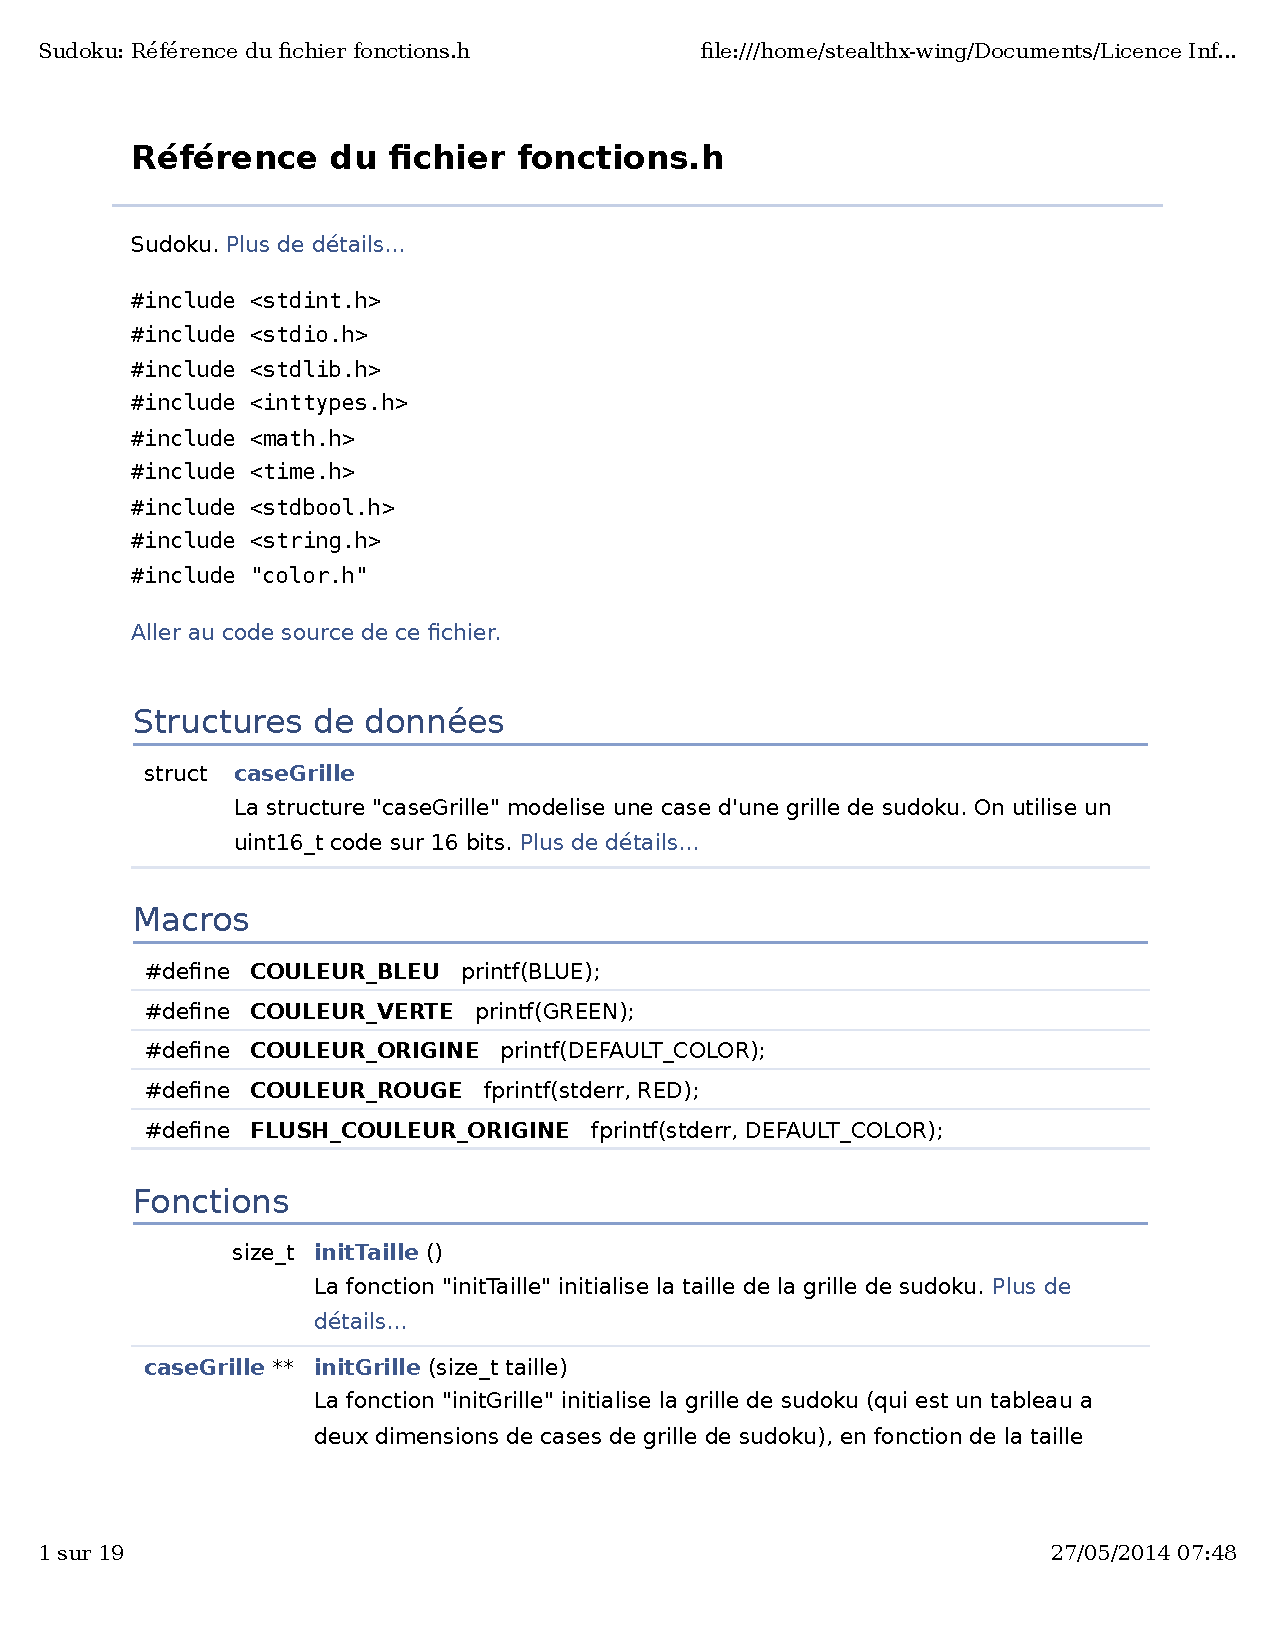
\includepdf[pages=1-16]{api}

	\newpage
	\strut
	\newpage

\end{document}
